\documentclass[../rapport.tex]{subfiles}
\graphicspath{{\subfix{ressources/}}}

\begin{document}
	
	\begin{figure}[h]
		\centering 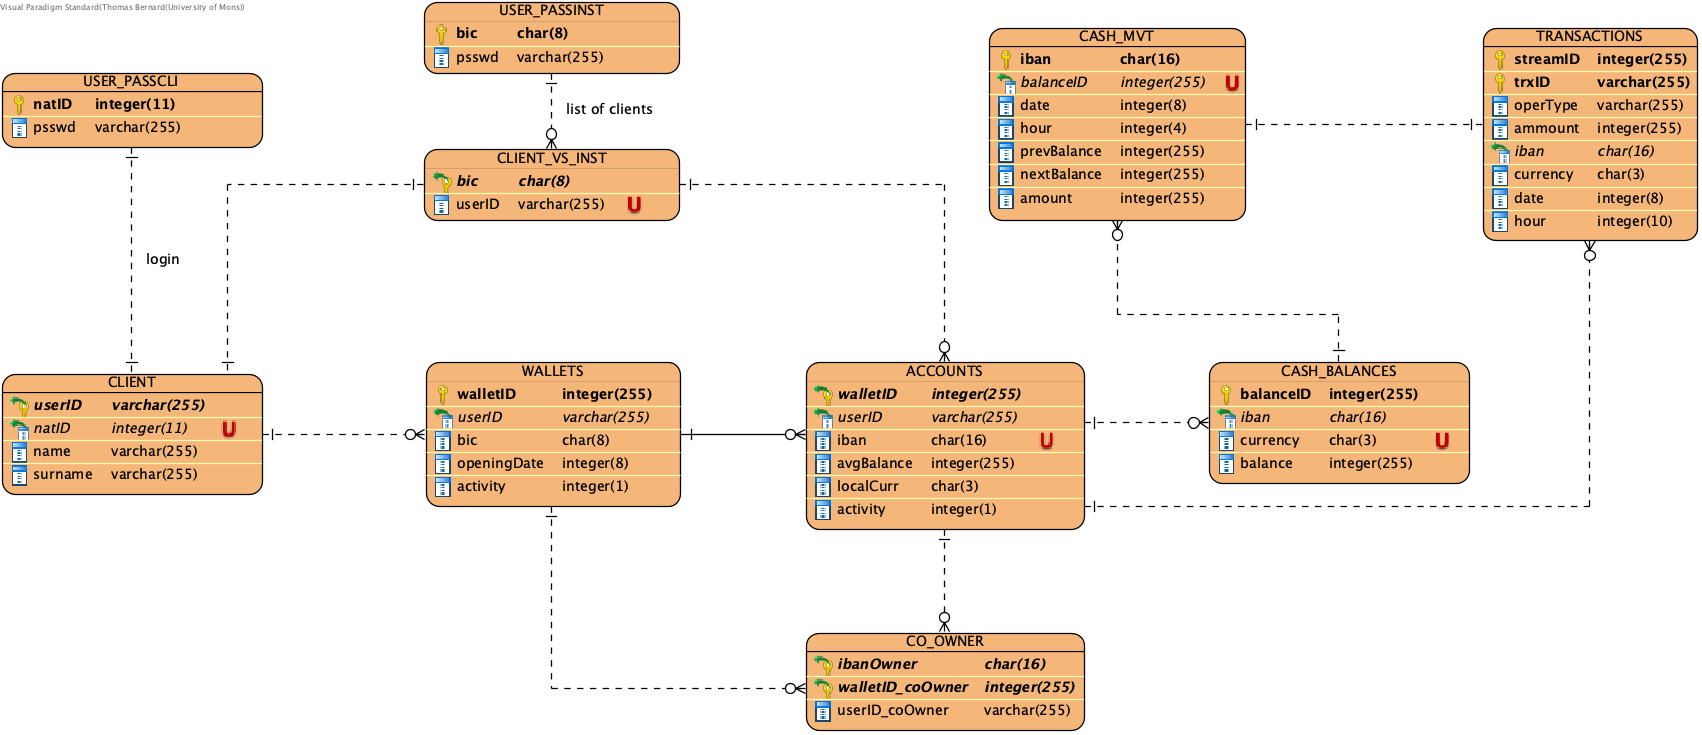
\includegraphics[scale=0.5]{erd.png}
		\caption{Diagramme d'entité-relation de l'application.}
	\end{figure}
	
	\paragraph{Tables utilisateurs :}
	Pour notre base de données nous avons essayé de séparer au mieux les tables afin que celles-ci restent simples de compréhension et faciles d'accès. Nous avons une table \textbf{USER\_PASSCLI} qui sert de table d'authentification. Elle contient le mot de passe \textbf{psswd} ainsi que le numéro de registre national de l'utilisateur \textbf{natID} si les deux correspondent alors on peut accéder à la table \textbf{CLIENT} qui contient quant à les informations personnelles du client ainsi que son nom d'utilisateur \textbf{userID}.
	
	\paragraph{Tables des institutions :} Afin que les insitutions n'aient pas accès à la notion de portfeuilles nous avons introduit 2 tables qui leurs sont propres et qui permettent de faire le lien entre les clients de la table CLIENT et leurs produits financiers de la table ACCOUNTS.
	
	\medskip
	
	La table \textbf{USER\_PASSINST} est à l'image de la table \textbf{USER\_PASSCLI} une table d'authentification pour les institutions à l'aide de leur identifiant \textbf{bic}. 
	

\end{document}